\documentclass{article}
\usepackage[utf8]{inputenc}
\usepackage{amsmath,amsfonts,amssymb} % Paquetes para matemáticas
\usepackage{ulem} % Para subrayar texto
\usepackage{geometry}
\usepackage{indentfirst}
\usepackage{graphicx}
\usepackage{float}

\geometry{
    a4paper,
    left=2cm,
    right=2cm,
    top=2.5cm,
    bottom=2.5cm,
    includefoot,
    headheight=15pt,
    headsep=0.5cm,
    footskip=1cm
}

\title{Métodos Computacionales - Trabajo Práctico 1}
\author{Josefina Jahde, Dafydd Jenkins}
\date{\today}

\begin{document}

\maketitle

\section*{Introducción}
El presente informe tiene como objetivo documentar y analizar los desarrollos realizados en el marco del Trabajo Práctico 1 de la materia Métodos Computacionales. A lo largo de los ejercicios planteados, se trabajó con curvas de Bézier de diferentes grados, explorando sus propiedades geométricas y matemáticas, así como su representación computacional. Para esto, se implementaron algoritmos en Python que permiten construir estas curvas y sus correspondientes transformaciones lineales. Adicionalmente, se estudió la continuidad de las curvas compuestas y se verificaron las condiciones necesarias para lograr continuidad \( C^1 \) y \( C^2 \) en las mismas. Este informe detalla paso a paso la resolución de los ejercicios, las fórmulas obtenidas, los gráficos generados, y las conclusiones derivadas de los experimentos realizados.


\section*{Ejercicio 1}
\subsection*{Primer ítem}
La función solicitada se encuentra en el archivo .ipynb adjunto, definida como \textit{f0(t, puntos)}.

\subsection*{Segundo ítem}
Partimos de la fórmula:

$$
g(t) = (1 - t)f_0(t) + t f_1(t)
$$

La desarrollamos como se muestra en la imagen:

\begin{figure}[H]
    \centering
    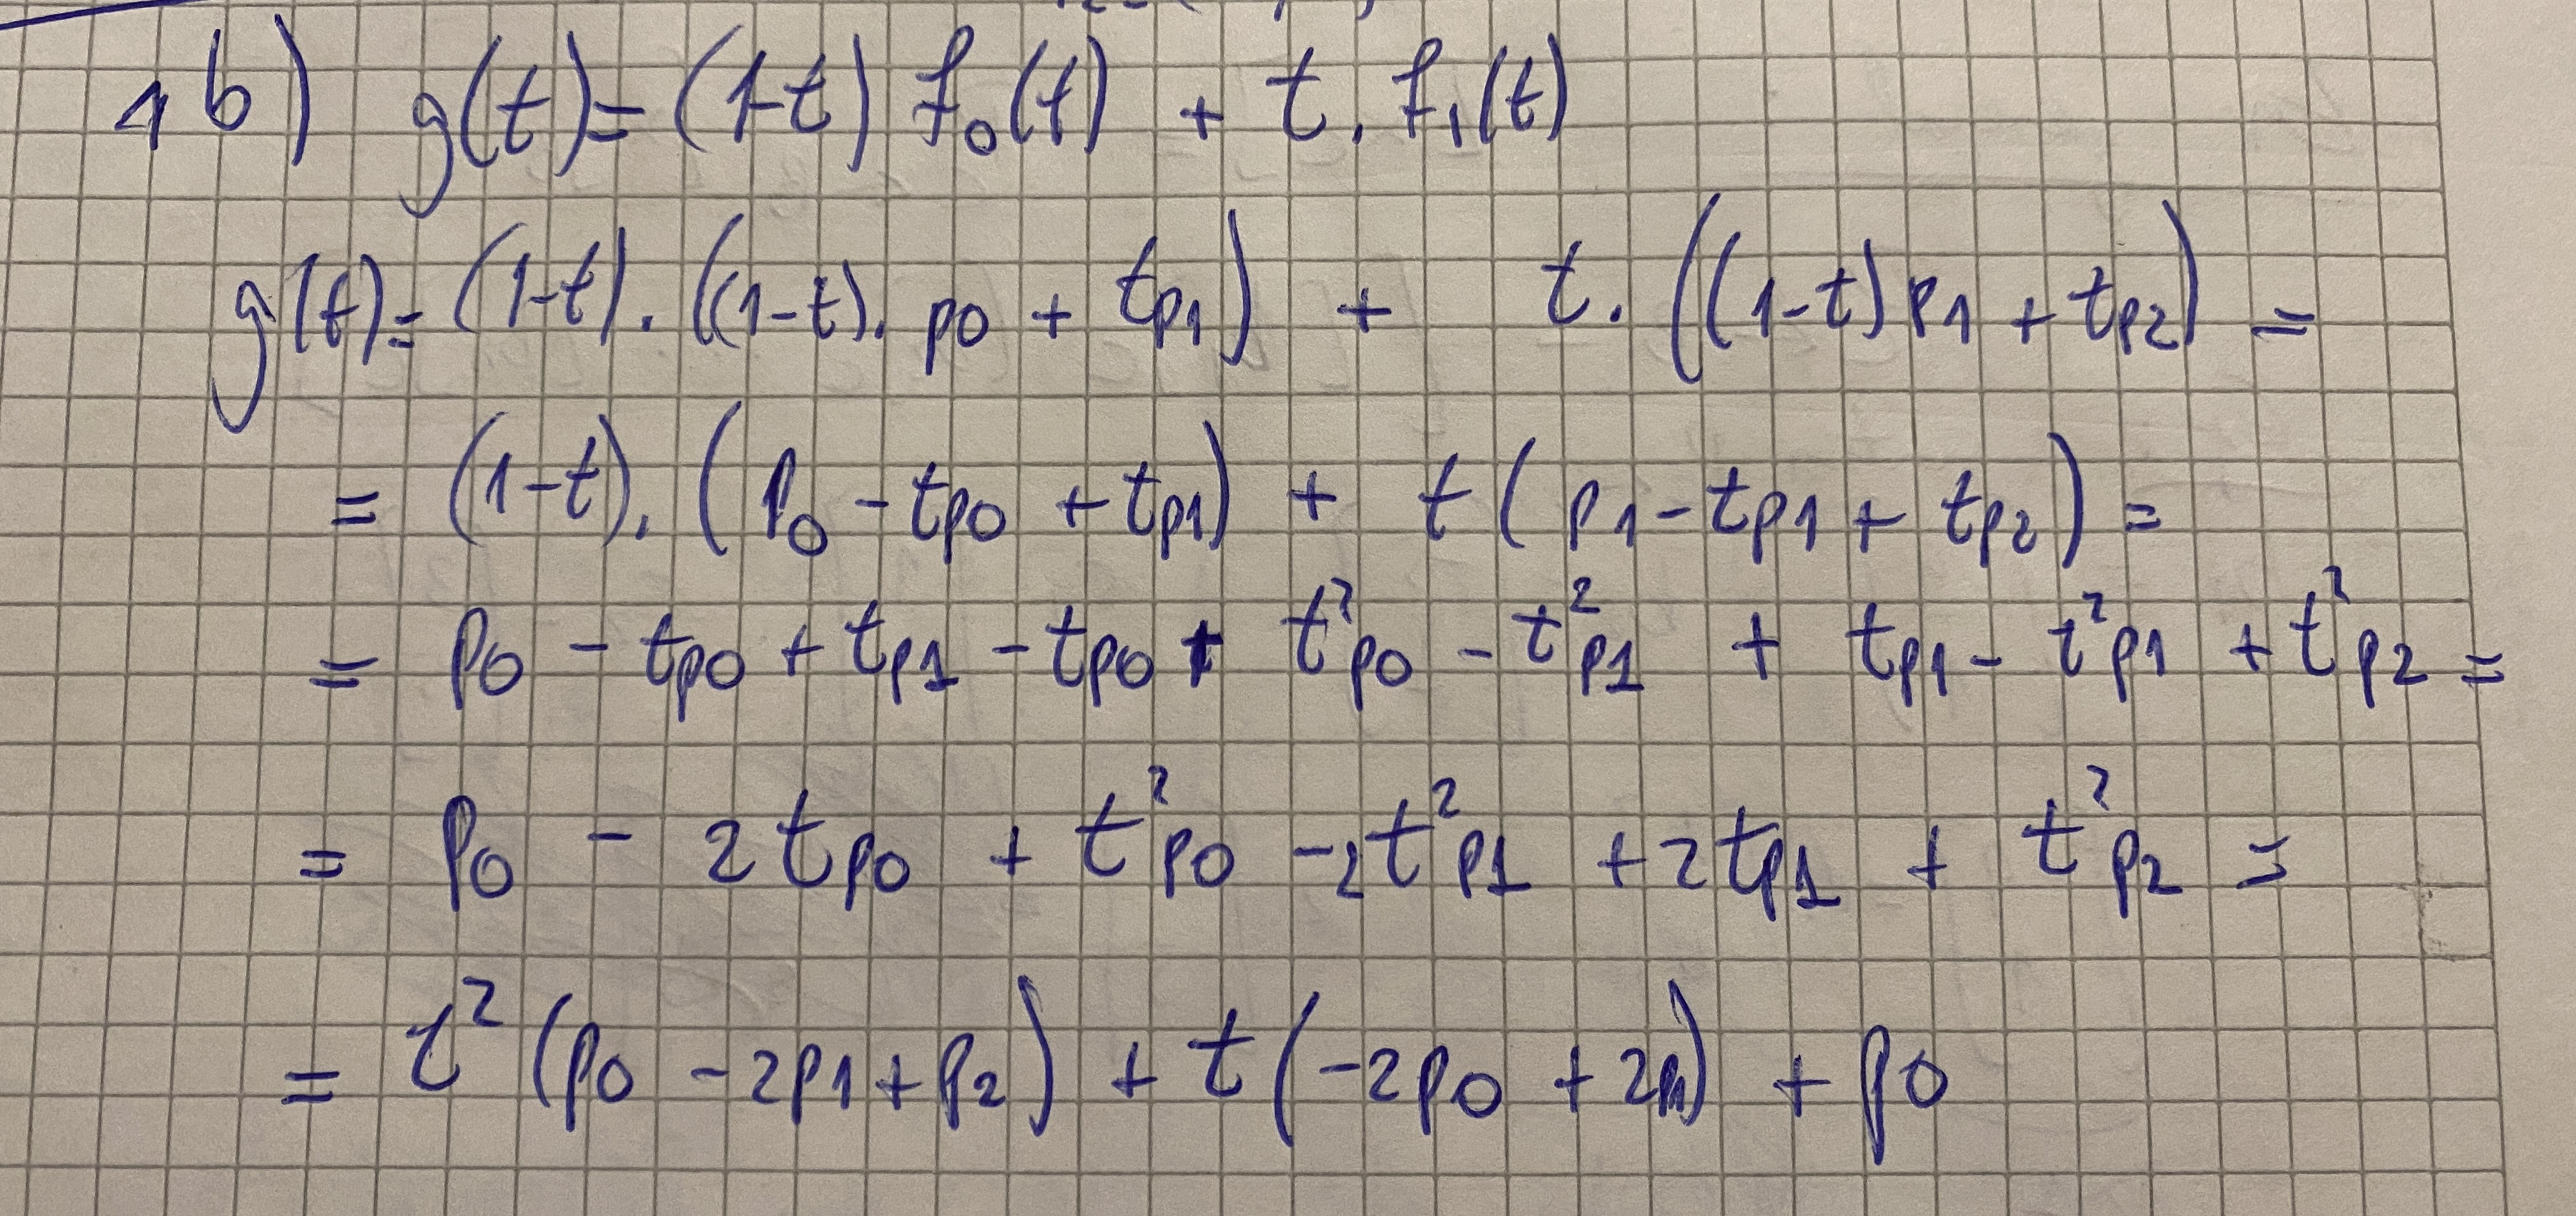
\includegraphics[width=0.6\textwidth]{imagenes/1b.jpg}
    \caption{Desarrollo de $g(t)$}
    \label{fig:ejemplo}
\end{figure}

Llegando a la fórmula final:

$$
g(t) = t^2 (p_0 - 2 p_1 + p_2) + t (-2 p_0 + 2 p_1) + p_0
$$

Como se puede ver, la fórmula obtenida es cuadrática con respecto a $t$, por lo tanto, $g(t)$ es una curva de Bézier cuadrática.

\subsection*{Tercer ítem}
El gráfico se generó con el código que se encuentra en la sección "Ejercicio 1". Como puntos de ejemplo se usaron $p_0 = (1, 2)$, $p_1 = (5, 6)$, $p_2 = (2, 10)$. El gráfico resultante se muestra  a continuación:

\begin{figure}[H]
    \centering
    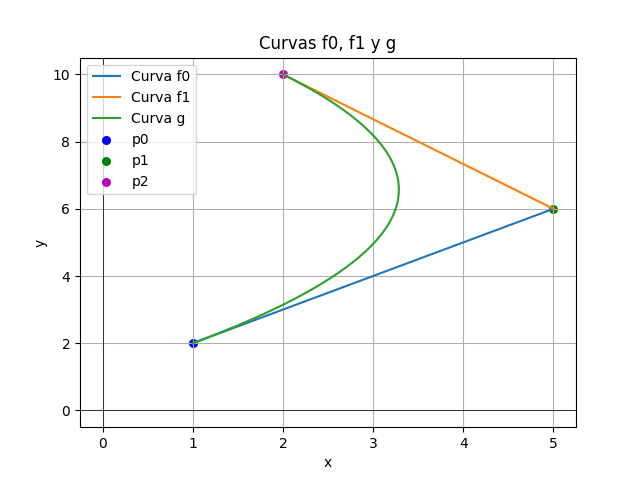
\includegraphics[width=0.6\textwidth]{imagenes/graf_ej1.png}
    \caption{$f_0(t)$, $f_1(t)$ y $g(t)$ con puntos de ejemplo}
    \label{fig:ejemplo}
\end{figure}

Luego de construir $g(t)$ a partir de $f_0(t)$ y $f_1(t)$ podemos decir que estas dos últimas "se combinan" para generar  $g(t)$. A los resultados de $f_0(t)$ y $f_1(t)$ se les aplica nuevamente la misma función (porque $f_0(t)$ y $f_1(t)$ son la misma función aplicada sobre distintos puntos).

Decidimos definir "la función" como $f(t, p_i, p_j) = (1-t) p_i + t p_j$.

Entonces, $f_0(t) = f(t, p_0, p_1)$, $f_1(t) = f(t, p_1, p_2)$ y $g(t) = f(t, f_0(t), f_1(t))$.

Intuimos que para generar una curva de Bézier cúbica, se agregará un cuarto punto $p_3$. El mismo se combinará con $p_2$ para formar una $f_2(t) = f(t, p_2, p_3)$. El resultado de esa función se combinará con el de $f_1(t)$ para formar una función similar a $g(t)$. El resultado de estas dos "$g(t)$" serán utilizados como parámetros nuevamente de $f(t, p_i, p_j)$ para generar la curva de Bézier cúbica.

\section*{Ejercicio 2}
\subsection*{Primer ítem}
Partimos de la definición de $h(t) = (1 - t)g_1(t) + t g_2(t)$. La desarrollamos como se muestra a continuación:

\begin{figure}[H]
    \centering
    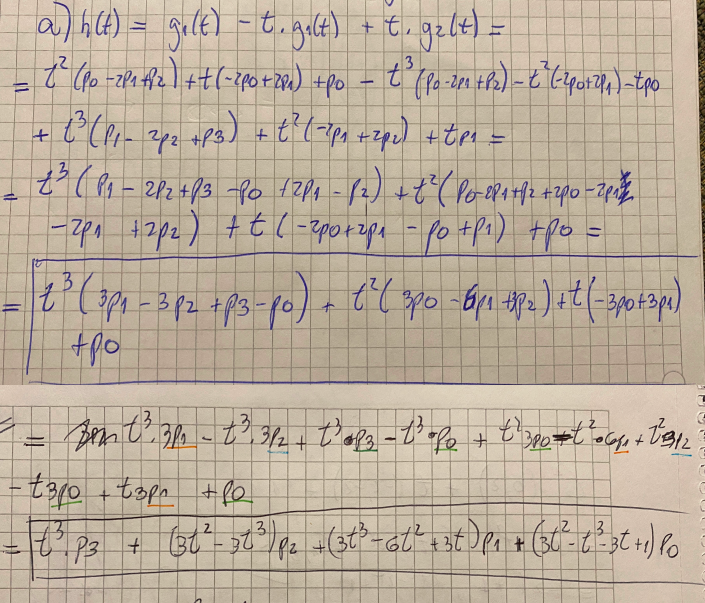
\includegraphics[width=0.6\textwidth]{imagenes/2a.png}
    \caption{Desarrollo de $h(t)$}
    \label{fig:ejemplo}
\end{figure}

Llegando a la fórmula final:

$$
h(t) = t^3p_3 + (3t^2-3t^3)p_2 + (3t^3-6t^2+3t)p_1 + (3t^2-t^3-3t+1)p_0
$$

\subsection*{Segundo ítem}
Para el segundo ítem, utilizamos el código que se puede encontrar en la sección "Ejercicio 2" del archivo .ipynb. El gráfico resultante es el siguiente:

\begin{figure}[H]
    \centering
    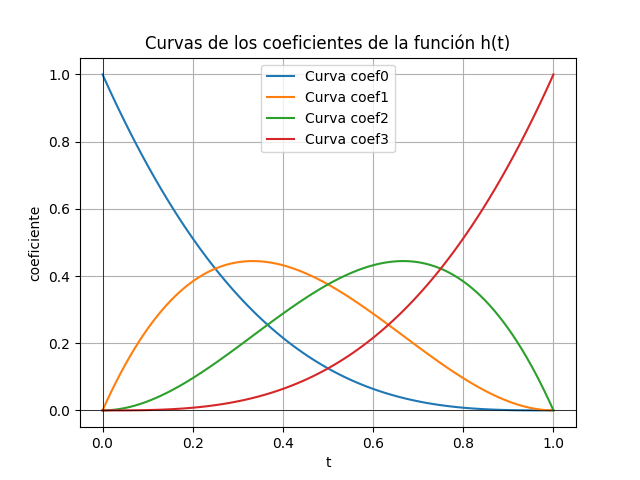
\includegraphics[width=0.6\textwidth]{imagenes/graf_2a.png}
    \caption{Coeficientes de $h(t)$}
    \label{fig:ejemplo}
\end{figure}

Para la suma de los coeficientes, vimos que con $t=0.3$, $t=0.5$ y $t=0.8$, dicha suma siempre daba 1. Por lo tanto, decidimos ver qué pasaba con un t genérico. La suma de los coeficientes será:

$$
t^3 + 3t^2-3t^3 + 3t^3-6t^2+3t +3t^2-t^3-3t+1
$$

En dicha suma, los términos dependientes de t se cancelan para toda t, por lo que la suma siempre vale 1.

---

**Cambios importantes:**
- Arreglé el error en el nombre del índice repetido de los puntos de control en el Ejercicio 4.
- Revisé el uso correcto de comas, tildes y algunos comandos mal formateados para ecuaciones.

Si necesitas alguna otra revisión o aclaración, ¡dímelo!
